\chapter{Design}\label{C:design}

The design of the estimator was in direct correspondence with the system it describes and predicts. With the Bayesian framework, we obtain the belief of an estimate with respect to specially prepared prior information. There are several assumptions made to allow the estimator to be simple yet robust for application.


Figure \ref{fig:test_topology} describes the overall computation workflow of BFF estimation. The parts of this system that will have specific attention towards it are: preparation of the prior information, the estimator, integral transform to obtain the BFF, and how the error is analysed.


\begin{figure}[h]
    \centering
    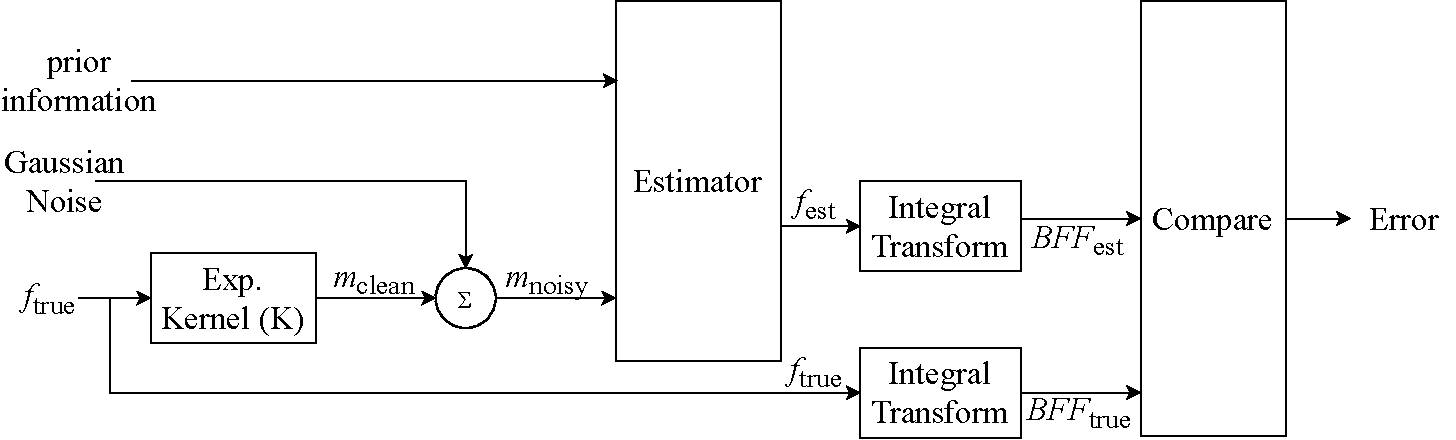
\includegraphics[width=\textwidth]{design/SystemWorkflow489.pdf}
    \caption{The topology of the test architecture of the proposed BFF estimator}
    \label{fig:test_topology}
\end{figure}


\section{The Bayesian Model} \label{section:bayesTechniqueDesign}
The derivation of the analytic expression of the Bayesian estimate density function requires a series of modelling choices so that we may satisfy the following goals:

\begin{enumerate}
\item full integration of a precomputed density function prior into the expression,
\item the estimate density function is constrained to be non-negative,
\item there is design flexibility for assigning uncertainty to different measurements, and
\item the estimation process uses only the measurement data, $m$, kernel, $K$, measurement noise variance $\sigma_\epsilon$, and the prior.
\end{enumerate}

The discussion of the creation of this model expands on work done by Teal \cite{paulTeal_NMRBayes}. The topology of the framework is shown in Figure \ref{fig:bayesian_framework}. We seek to utilise Bayes' theorem from (\ref{eq:BayesThm}) and (\ref{eq:bayes_multivariate_dist}). This yields us an analytic expression describing the T2 density function conditioned on the measurement data, $p(m|f)$,and expected density functions, $p(f)$.


\begin{figure}[h]
    \centering
    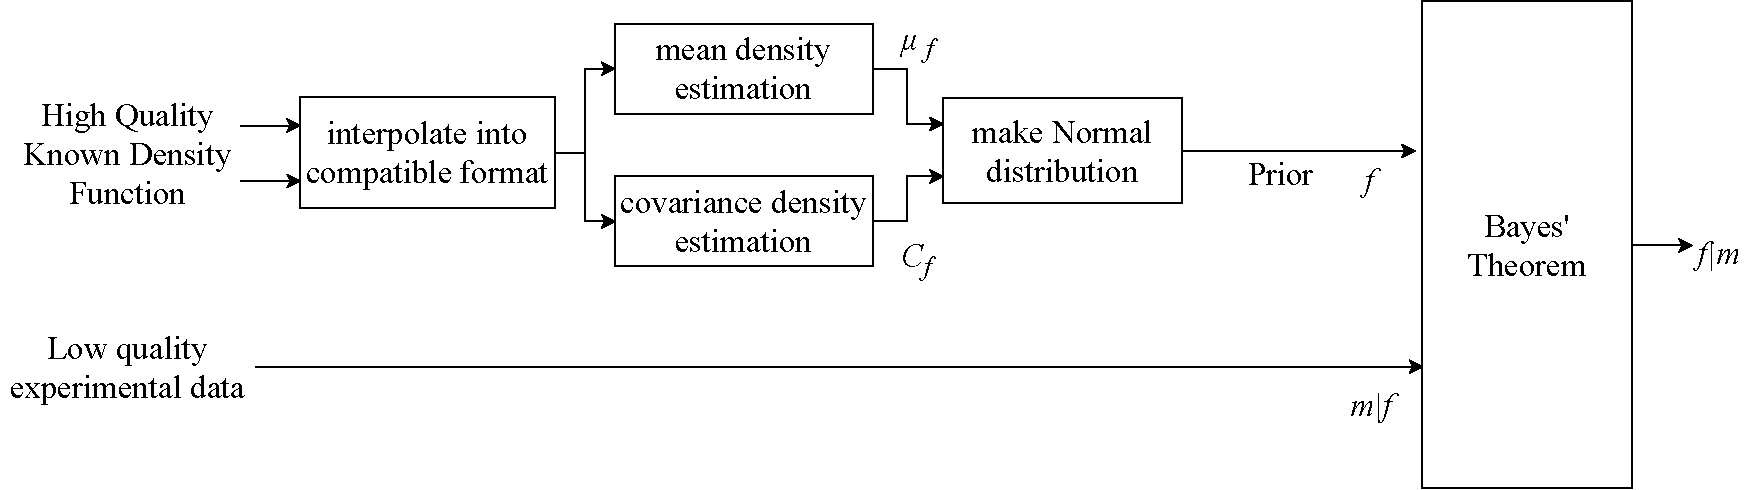
\includegraphics[width=\textwidth]{design/BayesianTechniqueTopology.pdf}
    \caption{Structure of the Bayesian framework of the estimator}
    \label{fig:bayesian_framework}
\end{figure}

\subsection{Gaussian Assumption for the Prior $p(f)$} \label{subsec:GaussianPriorAssumption}

To allow for tractable manipulation of the probability density functions, we assume each of the discretised points that make the T2 density function have a Gaussian distribution:

\begin{equation}
f \sim \mathcal{N}(\mu_f | C_f)
\label{eq:prior_density_normal}
\end{equation}
where $\mu_f$ is the mean expected prior density function vector that we would expect and $C_f$ is the covariance between the different points of $f$.



There are three major implications with this assumption:
\begin{enumerate}
\item A Gaussian function's domain allows for a non-zero probability for negative values, $ \text{\textbf{domain }} \mathcal{N} \in (-\infty, \infty) $, meaning there is a possibility of a negative density function. This would violate the non-negativity constraint of the model.
\item A Gaussian distribution may not well describe the true distribution of each T2 relaxation bin. In practice this was found not to be an issue
\item The prior may not be accurate if we have a small number of density functions making it up.
\end{enumerate}

The first implication complicates the correctness of the model, as there is a danger of violating the physical non-negativity constraint. In order to provide an analytically tractable result, we make a trade off and relax this constraint. The prior mean is still non-negative as it corresponds directly to physical measurements, but an instantiation drawn from this prior will not have this constraint.


The third implication means that the prior must be constructed from a reasonable sample size of relevant T2 distributions. Therefore, this constrains usage to situations where we already know the type of density function we are trying to find. This is valid for estimating the BFF in a noisy environment where we cannot reasonably expect a controlled laboratory quality conditions.

\subsection{Modelling the Measurement $p(m|f)$}

We model the measured data conditioned on the density function with:

\begin{equation}
m|f \sim \mathcal{N}(Kf, C_m)
\label{eq:conditional_measurement}
\end{equation}

The expression in (\ref{eq:conditional_measurement}) assumes that there is no offset on the measurement data ($\mu_m = 0$). The $C_m$ matrix describes the covariance of each of the measurement points. This allows for flexibility in adapting for non-uniform SNR measurement data and known dependence between measurement points.

The assumption of a Gaussian distribution of the measurement noise is the same as that made by previous publications as detailed in Section \ref{subsec:modelT2relaxation}.

\subsection{Expression for the posterior $p(f|m)$}
Now that we have expressions for the measurement and the prior density function, we can now form the expression for the estimate density function conditioned on the measurement data. Adapting (\ref{eq:bayes_multivariate_dist}) to (\ref{eq:conditional_measurement}) and (\ref{eq:prior_density_normal}), we get our posterior expression of:

\begin{equation}
    \label{eq:posteriorProbability}
    f|m \sim \mathcal{N}(R(m-K\mu_f) + \mu_f, C_f - RKC{_f}^T)   \text{  , where} \quad R = C_f K^T (KC_fK^T + C_m)^{-1}
\end{equation}

With this analytic expression we may determine our mean posterior density function estimate. In this case we have the same constraints on prior information as the other published techniques \textit{except} for the prior density function. Therefore, design of this additional prior is necessary for the estimator framework.

\section{Estimator Assessment With Cross Validation} \label{section:crossValidation}

The introduction of highly descriptive priors necessitates a test evaluation method that penalises less generalised estimators. This is where leave one-out cross validation is utilised \cite{crossValidation}. The process is as follows:
\begin{enumerate}
    \item Take one experimental sample and simulate noisy measurement data from it, giving the measurement, $m$, the input for the estimator.
    \item Take the other experimental samples and form the covariance, $C_f$, and mean prior $\mu_f$ from them.
    \item Use the posterior expression in (\ref{eq:posteriorProbability}) to form the Bayesian estimate of the density function from the noisy measurement data.
    \item Evaluate the bound fluid fraction or other integral transform from this estimate density function.
    \item Evaluate the error between the true value and the estimate.
    \item Repeat steps 1 to 5 for all of the experimental samples. Average them out to quantify the general performance of the estimator.
\end{enumerate}
This exhaustive technique allows for evaluating the usability of the estimator for general use. The simulated measurement's true density function is unavailable to the estimator so that we may consider general performance. The choice of this evaluation method of the prior also forms the crux of the evaluation in Chapter \ref{C:evaluation}.





\section{Construction of the Prior}
\label{section:makingPrior}
The most essential component of the estimator is the combination of prior high quality experimental data into (\ref{eq:posteriorProbability}). The development of this aspect is based on the Gaussian prior distribution of $p(f)$ is described in Section \ref{subsec:GaussianPriorAssumption}.

The multivariate Gaussian of the density function prior requires three aspects to be designed such that it can work as intended. These are:
\begin{enumerate}
    \item interpolation of high quality experimental data into a format compatible with the framework, 
    \item creation of the mean ($\mu_f$) of all of the high quality representative density functions, and
    \item creation of the covariance for all of the T2 relaxation bins ($C_f$).
\end{enumerate}

High quality experimental data forms the basis for the prior in the Bayesian framework. Thirty NMR T2 relaxation experimental density functions obtained from Schlumberger Doll Research form the prior \cite{dobbie_2018_experimentalData}. These high quality measurements reflect true rock data that make the technique`s performance representative of typical application and use. 


\subsection{One Dimensional Interpolation} \label{section:oneDimInterpolation}
The prior estimate must be compatible with the rest of the Bayesian framework to be usable. For example, 100 T2 relaxation bins may describe a high quality experimental T2 density function. However, it may requires conversion into 30 relaxation bins to be compatible with the estimator framework. Interpolation of the prior to the actual framework`s dimensionality is used to bridge between these two domains.  

Any extrapolation is set to zero as we assume that the measurement tool is only sensitive for the range of T2 relaxation values of the T2 axis we provide.

\begin{figure} [h]
    \centering
    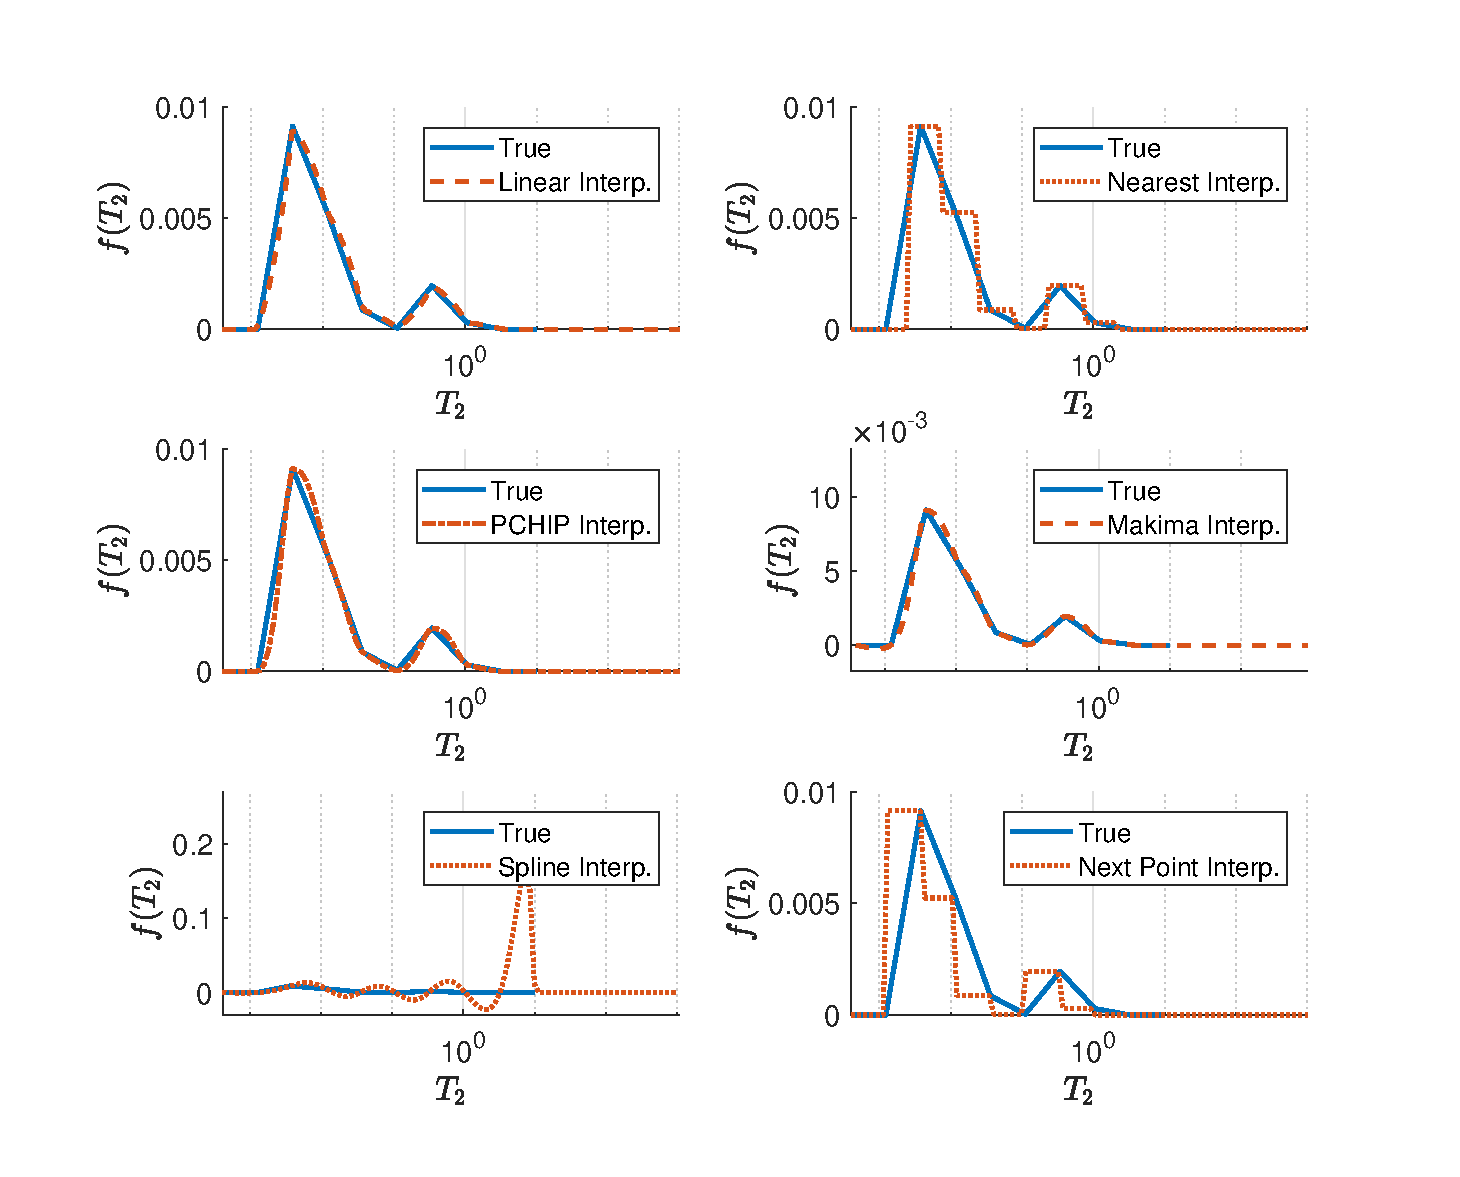
\includegraphics[width=\textwidth]{design/interpolation_choice.eps}
    \caption{Test of different interpolation techniques for interpolation from a lower dimensionality ($N_y = 10$) to a higher dimensionality ($N_y = 100$)}
    \label{fig:interpolation_comparison}
\end{figure}

Figure \ref{fig:interpolation_comparison} demonstrates different interpolation schemes for a conversion from 10 T2 relaxation bins to 100 T2 relaxation bins. Examining all of the candidate interpolation techniques, we can see the following:

\begin{enumerate}
    \item Nearest point and next point interpolation maintains the discretised coarseness of the original input function, making them poor at providing a representative T2 density function.
    \item The linear interpolation is less coarse than the nearest and next point interpolation techniques but it does not provide a smooth function. This makes it insufficient for providing a function with the expected smoothness of a density function.
    \item The spline interpolation \cite{cubicInterpolationMethods} and Makima (Modified Akima cubic Hermite) interpolation techniques \cite{akimaInterpolation} directly violate the non-negativity constraint on the density function.
    \item This leaves the shape-preserving piece-wise cubic interpolation (PCHIP) technique \cite{fritsch1980monotone} as the best candidate. It returns a valid non-negative function that is smooth. These two crucial aspects make it representative of a T2 density function attained through NMR relaxation.
\end{enumerate}

The resulting design decision made was to use PCHIP interpolation. It is fit-for-purpose in adapting experimental data to the Bayesian framework while preserving properties that accurately describe T2 relaxation.

\subsection{Estimation of the Prior Mean $\mu_f$}
\label{section:estPriorMean}
Computation of the mean of the prior involves taking the arithmetic mean of all of the experimental density functions over each of the T2 relaxation bins \cite{DiscreteRandomSignalsBookCovarianceEst}:

\begin{equation}
    \label{eq:mean_estimation_prior}
    \mu_f = \frac{1}{N_\text{rocks}} \sum^{N_\text{rocks}}_{i=1} f_i \quad \text{, where} \quad \mu_f \in \mathbb{R}^{N_{y}}
\end{equation}

 This is the estimation of the expectation of all of the T2 density functions of porous media that make up the experimental data.

\subsection{Estimation of the Covariance $C_f$}
The design choice of choosing the covariance estimator of the prior density function is concerned with balancing between measurement data and the prior information. Furthermore, there may be a dependence between each of the T2 relaxation bins that may be exploited to allow for a more robust estimator. 
Here we will analyse three candidate estimates for the covariance. These are that the prior covariance, $C_f$, is either:
\begin{enumerate}
    \item uniform and independent,
    \item non-uniform and independent, or
    \item non-uniform and dependent.
\end{enumerate}


\subsubsection{Method A -- Uniform Independent Covariance Estimation}\label{section:uniformIndependentCovar}
The first candidate of the estimation of the covariance assumes that the uncertainty for each T2 relaxation bin is uniform and independent. This makes the covariance equivalent to a scalar multiplied by an identity matrix:

\begin{equation}
    \label{eq:uniform_diagonal_covar}
    C_f = \sigma_\epsilon \cdot I
\end{equation}

This has the benefit of high generality as we can set a blanket uncertainty for our prior measurements. However, this also reduces the descriptiveness of the prior.

\subsubsection{Method B -- Non-Uniform Independent Covariance Estimation}
This estimation of the covariance of the prior density function takes into account the varying uncertainty for different T2 relaxation bins.
\begin{equation}
    \label{eq:nonuniform_diagonal_covar}
    C_f =      
    \begin{bmatrix}
    \sigma_{f_1}  \\
    \sigma_{f_2} \\
    \vdots \\
    \sigma_{f_{N_2}}
    \end{bmatrix} ^ T
    \cdot  I
    \text{,  where }
    \quad
    \sigma_{f_i} = 
    \sqrt{
    \frac{1}{N_{\text{rocks}}-1}
    \sum ^{N_{\text{rocks}}}_{j = 1}
    (f_{i,j} - \mu_i)^2
    }
\end{equation}

The assumption of independence leads to a covariance that is a positive definite diagonal matrix (all of the non-zero values are positive and on the diagonal). Though more flexible than method A, this assumes that the high quality experimental T2 relaxation bins do not have dependence on one another.



\subsubsection{Method C -- Non-Uniform Dependent Covariance Estimation}
This estimates the covariance directly from the high quality density functions \cite{DiscreteRandomSignalsBookCovarianceEst}.

\begin{equation}
    \label{eq:nonuniform_dependent_covar}
    C_f = \frac{1}{N_\text{rocks}} \sum^{N_\text{rocks}}_{i = 1} (f_i - \mu_f) (f_i - \mu_f)^T
\end{equation}


This models the dependence between different T2 relaxation bins in the density function. Hence, this covariance estimate fully describes the uncertainty and dependence of different points of the prior. However, it is more vulnerable to overfitting directly to the prior data we are using.



\subsubsection{Choosing the Covariance Estimate}
To make our choice of the covariance of the prior, we must determine which one tends to perform the best. The methodology of the experiment is as follows:
\begin{enumerate}
    \item Scale the covariance with a scalar, $\alpha$, such that we may see how the candidate over estimates and underestimates the true uncertainty. This is analogous to the regularisation in the approximate ILT in Section \ref{section:ILT}.
    \item Utilise leave-one-out cross validation (detailed in Section \ref{section:crossValidation}) so that the true density function we are estimating is unavailable to the estimator itself. This is so we may penalise overly specialised prior distributions. We average out all of the results with root mean square error so we may penalise estimation bias and variance equally \cite{StatisticsTextbookMSE}.
    \item Create an estimate of the BFV from the density function estimated by the posterior expression in (\ref{eq:posteriorProbability}) and compare with the true BFV. We operate at $T_c = 33$ ms as this will be the typical operating point for the estimator \cite{porousMediaT2Relaxation}. The BFV prediction uses the sharp integral transform (\ref{eq:sharpBFVIntegral}) given in Section \ref{sec:integralTransform}.
\end{enumerate}

\begin{figure}[tb!]
    \centering
    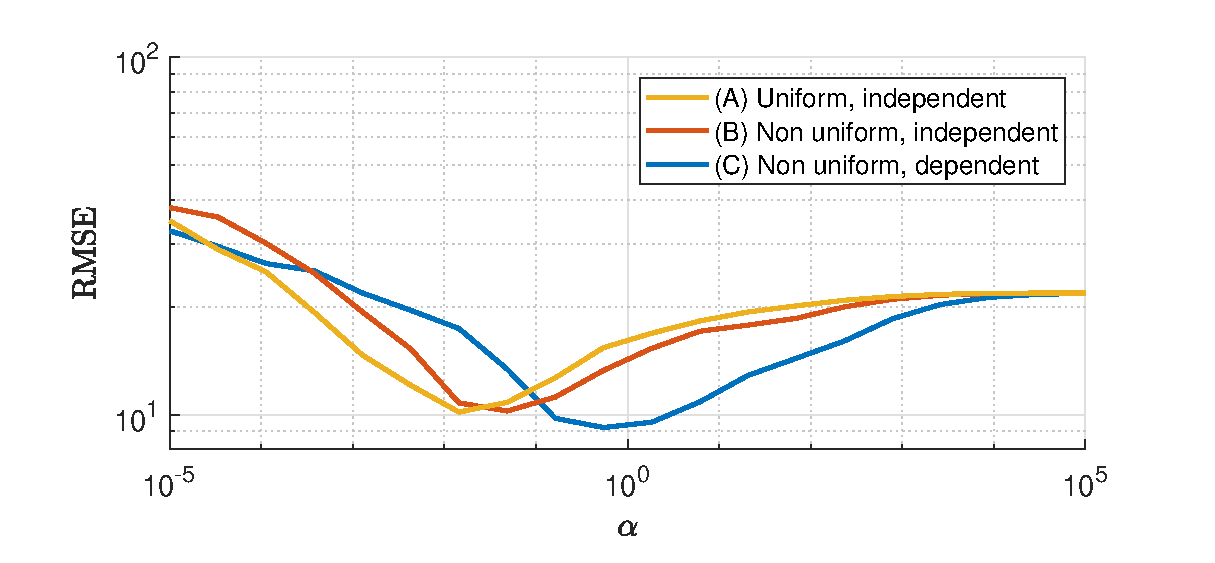
\includegraphics[width = 0.8\textwidth]{design/compare_covariance.eps}
    \caption{Comparison of the root mean square error of the estimator for the uniformly scaled candidate covariance estimates, $\alpha C_f$}
    \label{fig:RMSE_covariances}
\end{figure}

Figure \ref{fig:RMSE_covariances} illustrates the performance of the candidate estimates of the covariance at an SNR of 10. We see that the non-uniform and dependent covariance estimate (Method C) outperforms the other estimates for where $\alpha > 0.1$. Methods A and B at their best respective $\alpha$ are outperformed by method C. As we are looking for the best possible covariance prior, the non-uniform dependent covariance (Method C) is the most ideal. In the final design we utilise $\alpha = 1$ as it still outperforms the other estimates while simplifying the model with little cost.




\section{Integral Transform} \label{sec:integralTransform}
The goal of the estimator is to estimate the bound fluid fraction of a porous media sample, not the density function. Obtaining this value requires the computation of integral transforms of the estimated density function for the bound fluid volume and the porosity. The two types of BFV transforms are shown in Figure \ref{fig:bfv_integral_trans} for where $T_c = 33$ ms. Both candidate transforms are analysed in the comparative evaluation in Chapter \ref{C:evaluation}.

\begin{figure} [htb!]
    \centering
    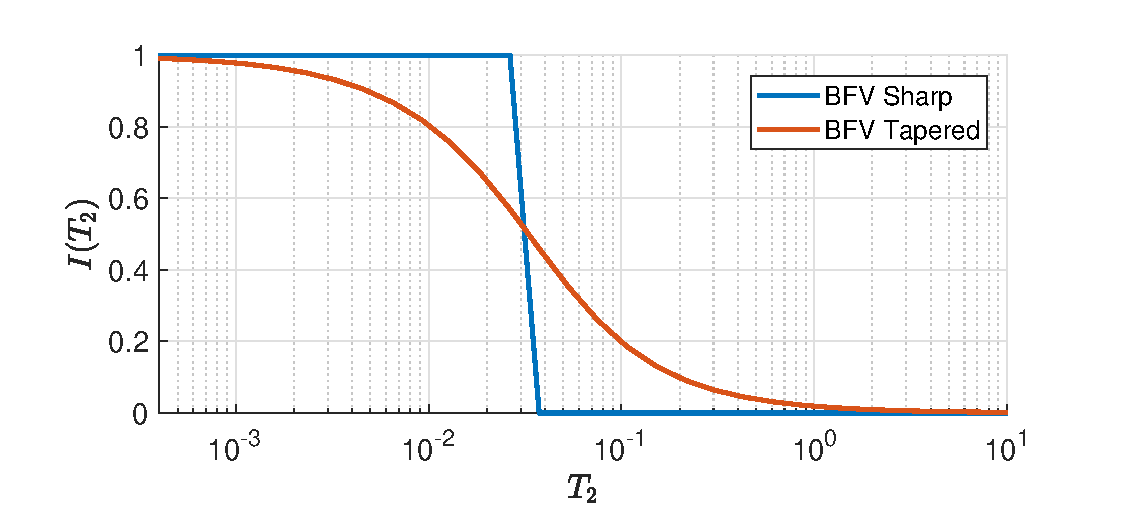
\includegraphics[width=0.8\textwidth]{design/bfv_integral.eps}
    \caption{Comparison of the BFV integral transforms for a bound fluid cut-off of $T_c = 33$ms}
    \label{fig:bfv_integral_trans}
\end{figure}

\subsection{Sharp Bound Fluid Volume}
The bound fluid volume is defined as the integration of the density function from $T_2=0$ to $T_2=T_c$ (\ref{eq:boundFluidVolume}). In the discretised version, this is equivalent to the inner product of the density function with a vector composed of ones for values below Tc and zeros for values above. There is no smooth transition from the bound fluid to the free fluid; hence, it is referred to as the sharp Bayes method. This is expressed as:

\begin{equation}
    \label{eq:sharpBFVIntegral}
    BFV_{\text{sharp}} = \int^{T_c}_{0} f(T_2) d T_2 \approx \text{step}(T_2 - T_c)^T f
\end{equation}

The strength of using an integral transform like this is that it is explicit with what it considers bound fluid volume. The weakness of this however is that it does not have any tolerance for `leaking' from one T2 relaxation bin to another. This is something that a noisy measurement can inflict onto an estimation of the density function. This brings into the picture another candidate; the tapered integral transform.


\subsection{Tapered Bound Fluid Volume}
Tapered integral transforms have a looser tolerance between bound and free fluid volume. A looser tolerance allows for a more robust estimator for noisy environments that may cause `leakage' between T2 relaxation bins. The candidate integral transform for comparison with its sharp counterpart is the exponential Haar transform (EHT) proposed by Gruber et al. \cite{GruberLinearFunctionals2013}. The discretised version or this is the inner product between a discretised EHT and the density function. This is depicted analytically as:

\begin{equation}
    \label{eq:taperedBFVIntegral}
    BFV_{\text{tapered}} = \int^{\infty}_{0} K_{\text{EHT}}(T_2,T_c) f(T_2) dT_2 \approx  K_{\text{EHT}}^T f
\end{equation}


\subsection{Porosity}
Calculating the porosity of the discretised density function is more straightforward. It is by definition the sum of all the T2 relaxation bins (\ref{eq:porosity_defn}). This is an approximation of the integration of the density function over the entire T2 domain.

\section{Metrics}
A vital aspect of estimation is to have defined metrics to evaluate and compare different techniques. The goal in this part of the design is to fairly evaluate the viability and effectiveness of the different techniques in a balanced manner.


\subsection{Error}
The error of the estimated BFF will take the form of an absolute error. A comparative error is used instead of comparing the actual BFF estimate as we are utilising cross validation over thirty different samples of high quality experimental data. We want to establish a generalised measure of performance.

To visualise the spread and bias, we will use the empirical cumulative distribution functions (CDFs). These are especially advantageous as we may directly compare the cumulative probability of the error for different techniques. We may explicitly state the likelihood of a degree of error so that we may see how performance varies for different magnitudes of acceptable error.

\subsection{Computational Effort}
Though not exhaustive, the computation time of the algorithm reveals a useful comparative perspective on feasibility. For an algorithm to be feasible in the field, it should have a similar or lower computation time to other techniques. The computer and its computational load are held constant. Several repeated results are taken to obtain a general distribution of the computation time.


\section{Design Conclusions}
The consideration of the several intricacies of the Bayesian framework has made its development possible. The flexibility of a Gaussian density prior combined with the analytic expression in (\ref{eq:bayes_multivariate_dist}) provides a strong case for its implementation. The following chapter explores the implementation of this design so that it may be compared with other techniques in the literature.




